\begin{figure}[h!]
    \centering
    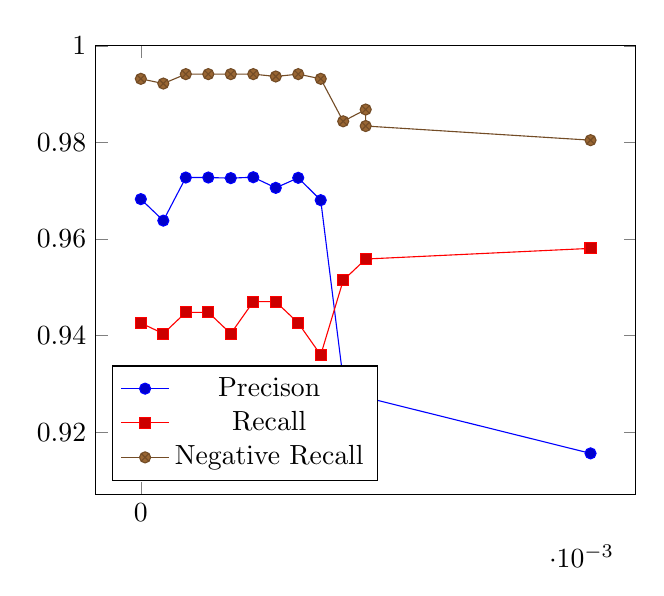
\begin{tikzpicture}
        \begin{axis}[
            legend pos=south west,
            ymax=1,
            xtick={0, 0.02, 0.04, 0.06, 0.08, 0.1},
            xticklabels={0, 0.02, 0.04, 0.06, 0.08, 0.1}
            ]
            \addplot+[sharp plot] coordinates {
            (0.000, 0.968254)
            (0.0001, 0.963801)
            (0.0002, 0.972727)
            (0.0003, 0.972727)
            (0.0004, 0.972603)
            (0.0005, 0.972789)
            (0.0006, 0.970588)
            (0.0007, 0.972665)
            (0.0008, 0.968037)
            (0.0009, 0.930886)
            (0.001, 0.927195)
            (0.002, 0.915612)
            };
            \addlegendentry{Precison}
            \addplot+[sharp plot] coordinates {
            (0.000, 0.942605)
            (0.0001, 0.940397)
            (0.0002, 0.944812)
            (0.0003, 0.944812)
            (0.0004, 0.940397)
            (0.0005, 0.947020)
            (0.0006, 0.947020)
            (0.0007, 0.942605)
            (0.0008, 0.935982)
            (0.0009, 0.951435)
            (0.001, 0.955850)
            (0.002, 0.958057)
            };
            \addlegendentry{Recall}
            \addplot+[sharp plot] coordinates {
            (0.000, 0.993161)
            (0.0001, 0.992184)
            (0.0002, 0.994138)
            (0.0003, 0.994138)
            (0.0004, 0.994138)
            (0.0005, 0.994138)
            (0.0006, 0.993649)
            (0.0007, 0.994138)
            (0.0008, 0.993161)
            (0.0009, 0.984367)
            (0.0010, 0.986810)
            (0.001, 0.983390)
            (0.002, 0.980459)
            };
            \addlegendentry{Negative Recall}
            %\draw[red,line width=1pt] ({axis cs:0.002,0}|-{rel axis cs:0,1}) -- ({axis cs:0.002,0}|-{rel axis cs:0,0});
        \end{axis}
    \end{tikzpicture}
    \caption{Precision and recall w.r.t. lower threshold (no cap on the upper bound)}
    \label{p:lowerbound}
\end{figure}


